\documentclass[9pt]{beamer}

\usepackage{préambule}
\usepackage{préambule-figures}
\usetikzlibrary{calc,positioning}

\begin{document}

\begin{frame}
	\begin{cours}[Vocabulaire du cylindre]
		\begin{center}
			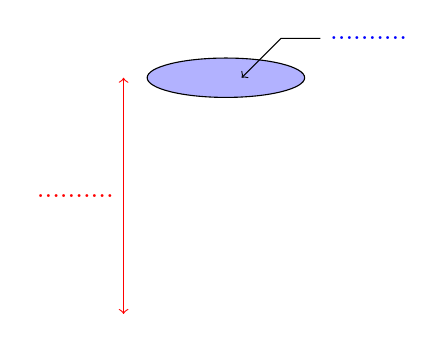
\begin{tikzpicture}
				\cylindre{3}{2}{0.5};
				\draw[draw=transparent,fill=blue!30] (0,0) ellipse (1 and 0.25);
				\draw[->] (1.2,0.5) node[right] {\color{blue}..........} -- ++(-0.5,0) -- ++(-0.5,-0.5);
				\draw[red,<->] (-1.3,0) -- node[midway,left] {\color{red}..........} ++(0,-3);
			\end{tikzpicture}
		\end{center}

		La figure ci-dessus est un .......... .
	\end{cours}
\end{frame}

\end{document}